%% Simple update
%
% A PEPS in the form simple update keeps it: a tensor Gamma on every site and a
% diagonal matrix lambda on every bond.
%
% The lambdas are the analogue of the Schmidt values of a chain, the centre on
% a bond, and they are drawn as it is. They are not exact here -- a lattice
% with loops has no canonical form -- but they are what the update uses as one:
% to apply a gate to a bond, absorb the lambdas around its two tensors, apply,
% split by SVD, keep the new singular values as the bond's lambda, and divide
% the old ones out again. Cheap, local, and approximate in exactly that way.
\documentclass[border=4pt]{standalone}
\usepackage{amsmath,amssymb}
\usepackage{tikz-tensors}
\input{notation}
\begin{document}
\begin{tikzpicture}
  \tngrid[bonds=centrebond/$\lambda$]{S}{3}{3}{coef/$\Gamma$}
  \tnconnect{S}
  \tnopen{down}{S}
\end{tikzpicture}
\end{document}
